\documentclass{beamer}
\mode<presentation>{\usecolortheme{crane}}
\usetheme{Madrid}


\usepackage{graphicx}
\usepackage{xcolor}
\usepackage[utf8]{inputenc}
\usepackage{hyperref}
\hypersetup{
    colorlinks=true,
    linkcolor=blue,
    filecolor=magenta,
    urlcolor=cyan,
}

\title{CS633 Project: Parallel Debugger}
\author[Milind, Subhdeep]{Milind Luthra (150363) \and Subhdeep Saha (150732)}

\date{26 April 2019}

\AtBeginSection[]
{
  \begin{frame}{Table of Contents}
    \tableofcontents[currentsection]
  \end{frame}
}

\AtBeginSubsection[]
{
  \begin{frame}{Table of Contents}
    \tableofcontents[currentsubsection]
  \end{frame}
}

\begin{document}

\frame{\titlepage}

\section{Overview}

\subsection{Motivation}
\begin{frame}
  \frametitle{Motivation}
  \begin{center}
      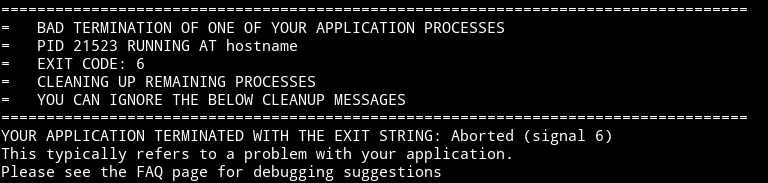
\includegraphics[width=\textwidth]{motivation}
  \end{center}
\end{frame}

\subsection{Related Work}

\begin{frame}
  \frametitle{Allinea DDT and Totalview}
  \begin{itemize}
  \item <1-> Debuggers already in use to debug large parallel applications.
  \item <2-> Both have a rich feature set and GUIs.
  \item <3-> However, both are proprietary, commercial software.
  \item <5-> Restrictive licenses (locked to one node, or four processes etc) and high cost (a few hundred dollars).
  \item <6-> Can't be extended any further.
  \end{itemize}
\end{frame}

\begin{frame}[fragile]
  \frametitle{Using XTerm and GDB}
  \begin{itemize}
  \item <1-> Possible Idea: For n processes, launching n XTerm instances with gdb.
  \item <2-> Each terminal can be used to debug the individual processes.
  \item <3-> \texttt{mpiexec -n 4 xterm -e gdb ./test}
  \end{itemize}
\end{frame}

\begin{frame}
  \frametitle{Problems with XTerm + GDB}
  \texttt{mpiexec -n 30 xterm -e gdb ./test}

  \begin{center}
    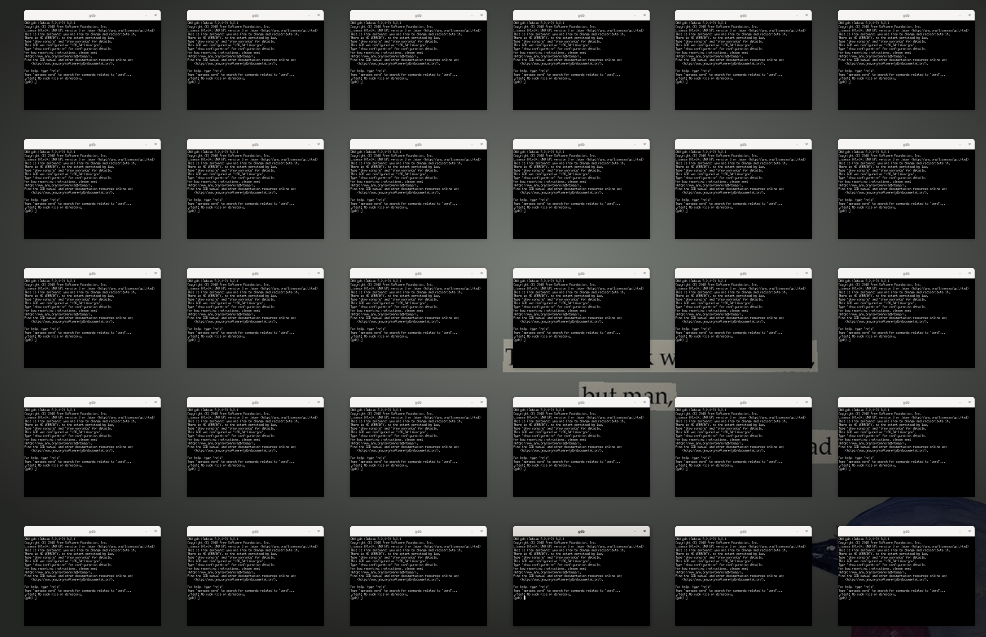
\includegraphics[width=0.9\textwidth]{usingxterm}
  \end{center}
\end{frame}


\subsection{Idea}
\begin{frame}
  \frametitle{Basic Idea}
\begin{itemize}
  \item <1-> The basic idea is to launch a number of clients on nodes using \texttt{mpiexec}.
  \item <2-> Each client instance will run a \texttt{gdb} instance with the program to be debugged.
  \item <3-> All the instances of \texttt{gdb} are controlled using a single, centralized interface.
\end{itemize}
\end{frame}

\section{Timeline}
\begin{frame}
  \frametitle{Timeline}
  \begin{itemize}
  \item <1-> Load and then instrument target binary in all nodes. \textsc{Done}
  \item <2-> Communicate with \texttt{gdb/mi}. \textsc{Done}
  \item <3-> Set up client and server communication (extract rank/size from instrumented binary). \textsc{Done}
  \item <4-> Allow commands from server to all clients, and echo client console on server. \textsc{Done}
  \end{itemize}
\end{frame}

\begin{frame}
  \frametitle{Timeline}
  \begin{itemize}
  \item <1-> Allow sending commands from server to only specific clients \textsc{\color{green} Done}
  \item <2-> Make a nice TUI. \textsc{\color{green} Done}
  \item <3-> Track communicator data. \textsc{\color{red} NotDone} (we tried this, problems explained later.)
  \item <4-> Track collective calls. \textsc{\color{green} Done} (for \texttt{MPI\_COMM\_WORLD})
  \item <5-> Track asynchronous call buffers. \textsc{\color{red} NotDone}
  \end{itemize}
\end{frame}

\section{Implementation}
\begin{frame}
  \frametitle{Architecture Overview}
  \centering
  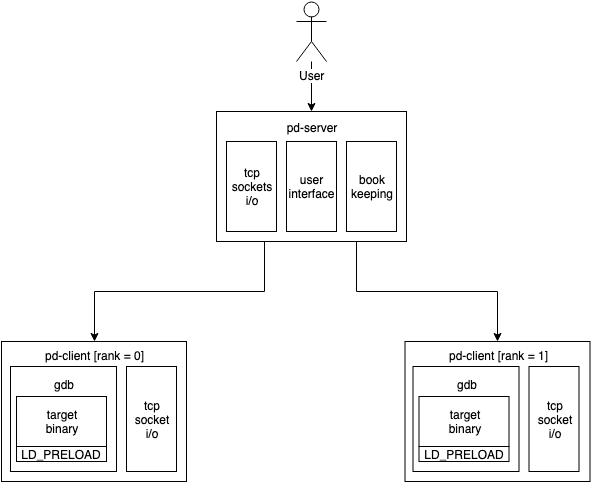
\includegraphics[width=0.8\textwidth]{overview}
\end{frame}

\subsection{Start-up Instrumentation}

\begin{frame}
  \frametitle{Starting Up}
  \begin{itemize}
  \item <1-> When the \texttt{pd-client} starts up, it starts an instance of \texttt{gdb}.
  \item <2-> The \texttt{gdb} instance loads the target binary, adding to \texttt{LD\_PRELOAD} our custom library.
 \item <3-> We write our own version of \texttt{MPI\_Init} inside our custom library.
 \item <4-> This consists of a call to \texttt{PMPI\_Init}, followed by writing the rank and the world size of \texttt{MPI\_COMM\_WORLD} to disk.
 \end{itemize}
\end{frame}

\begin{frame}
  \frametitle{Starting Up}
  \begin{itemize}
  \item <1-> The \texttt{gdb} instance sets a breakpoint on this custom function.
  \item <2-> Then, we run the program till this breakpoint is hit, and move to the end of the function.
  \item <3-> We extract the necessary information from the file, and send it to the server.
  \item <4-> Finally, the server sends acknowledgement when all clients are connected.
  \item <5-> When \texttt{MPI\_Init} ends, all the clients are connected to the server.
 \end{itemize}
\end{frame}

\subsection{Collective Call Tracking}
\begin{frame}
  \frametitle{C Code}
 \begin{itemize}
 \item <1-> For all the collectives we ever want to track, we add them to the library we are loading at runtime using \texttt{LD\_PRELOAD}.
 \item <2-> A ``marker'' function is inside each of the collectives we ever intend to instrument.
 \item <3-> Then, the MPI collective function sets up some variables to extract rank and communicator info, and calls the corresponding PMPI function.
 \item <4-> We use \texttt{volatile} to ensure that these functions/variables are not optimized out.
 \item <5-> Easy to add new MPI collectives - just two lines of code.
 \end{itemize}
\end{frame}

\begin{frame}
  \frametitle{Go Code}
  \begin{itemize}
  \item <1-> We can toggle tracking a particular collective with \texttt{pdb\_trackcoll <collective\_name>}.
  \item <2-> Once we begin tracking a collective, the Go code for the client (the one which controls \texttt{gdb}) sets a breakpoint on the ``marker'' function.
  \item <3-> On hitting that breakpoint, we extract rank and communicator, and then resume the running of the collective.
  \item <4-> This is completely transparent to the user.
  \item <5-> At any point the user can view pending collectives using \texttt{pdb\_listcoll}.
 \end{itemize}
\end{frame}

\subsection{Communicator Tracking}
\begin{frame}
  \frametitle{Idea}
  \begin{itemize}
  \item <1-> Each \texttt{MPI\_Comm} is actually an integer.
  \item <2-> Whatever function can create a new communicator, write a wrapper for it in our custom library.
  \item <3-> Break on that wrapper and extract communicator ID and rank of process transparently.
  \item <4-> Hence, we know which process belongs to the newly created communicator.
 \end{itemize}
\end{frame}

\begin{frame}
  \frametitle{Issues}
  \begin{itemize}
  \item <1-> \texttt{MPI\_Comm} integer representation is \textbf{not the same across processes}.
  \item <2-> Makes it hard to identify communicators uniquely and see what ranks (with respect to \texttt{MPI\_COMM\_WORLD}) are included.
  \item <3-> Alternative: trying to understand the \href{https://wiki.mpich.org/mpich/index.php/Communicators_and_Context_IDs}{context} using rules set by the MPICH library.
  \item <4-> Alternative: using \texttt{MPI\_Bcast} to send random integer from zero rank of new communicator and all the processes which send the same integer to the server can be grouped together.
 \end{itemize}
\end{frame}


\section{Demonstration}

\section{References}
\begin{frame}
  \frametitle{References}
  \begin{itemize}
  \item \href{https://sourceware.org/gdb/onlinedocs/gdb/GDB_002fMI.html}{GDB/MI2 Documentation}
  \item \href{https://github.com/cyrus-and/gdb}{Go library for talking to GDB/MI} - \href{https://github.com/milindl/gdb}{Our modified version of the library}.
  \item \href{https://en.wikipedia.org/wiki/Allinea_DDT}{Allinea DDT}, \href{https://www.roguewave.com/products-services/totalview}{TotalView}
  \item \href{https://www.open-mpi.org/faq/?category=debugging}{OpenMPI FAQ for Parallel Debugging}
  \item \href{http://www.linux-mag.com/id/7210/}{Common MPI Programming Errors}
  \item \href{https://wiki.mpich.org/mpich/index.php/Communicators_and_Context_IDs}{MPICH Wiki: Communicators and Context IDs}
  \end{itemize}
\end{frame}

\end{document}